\chapter{Data Preparation}
In this chapter, we introduce the data we used in this project. 
Audio event list is a list of audible events that we labelled manually, we mainly separate events into four big categories. 
In each category, we enumerate some common audible events. 
Audio data is important for our training process, and we download them in some Sound Search Engines (SSEs) and apply some downloading restrictions on potential clips. 


\section{Audible Event List} 
There are already some research done on the task of building a taxonomy for audio sounds. 
An urban sound taxonomy has been built \cite{salamon2014dataset}, but it is focused only on urban environment, and the size of taxonomy is also kind of small, not having a large coverage. 
Another broad categorization of sound environments was proposed in \cite{brown2011towards}, which separate sound by broad environments. 
It has the limitation of not having specific audible events for real event detection. 
Hence, we based on the previous work, and proposed a new taxonomy for audible events. 
A new event list is then formed by extracting events from this taxonomy.  \\ 

We separate sounds basically into four groups: Human, Mechanical, Nature, and Other Sound. 
These four group are just a rough categorization of audible events we want to include, so the meaning of these labels are very broad to include as many specific events as possible. 
Under the Human group, sound events are further separated into Movement, and Non-Movement. 
The difference of the two groups is that Movement focuses on sound made by human under some moving condition, while the Non-Movement group may just be the sound generated by human in a static condition.
Mechanical group was then divided into Equipment, Transport, and Material, three groups. 
In the Equipment, basic things we used in life under office, living or construction environment are enumerated. 
Transport more or less contains the transportation vehicles seen in modern life. 
And some common materials are listed under the Material group. 
In the Nature categorization, Animal, Plant, Element are the three basic group. 
They respectively list the things in nature which may generate a sound. 
Finally, Signal and Instrument are put under Other Sound. 
They include common signals and musical instrument in life. 

\section{Audio Data}
The audio clips for the events in the eventlist we created are downloaded from SSE. 
There are many available SSEs for crawling sound clips, e.g., SoundJax\footnote{http://soundjax.com}, FindSounds\footnote{http://findsounds.com}, and Freesound\footnote{http://freesound.org}. 
We use all these SSEs to query the audio events and then download their corresponding clips. 
However, this downloading process is carried out with some filtering technique. 
Because the events we are considering suitable are "primitive" constituents for large audio context, their information should be covered in a comparative short time. 
So we set up a duration threshold for candidate audio clips, i.e., only downloading clips from 0.5 to 10 seconds.  

\section{Scene Context Data}
In some previous project, researchs are labelling the audible events happening in some scenes. 
This method is not only laborious, but also has a limitation for expanding to other scenes.
In this thesis, we are using a automatical way of extracting the relation between audible events and scenes.
The data we use are well-written scripts, including movies, plays, TV series, etc. 
The reason we use these scripts is because they all have a clear boundary of one "scene". 
In well-written scripts, whenever the plot switches to a new place, there is a sentence in the top to indicate what the current scene is. 
% script example
\begin{figure}[htb]
\centering
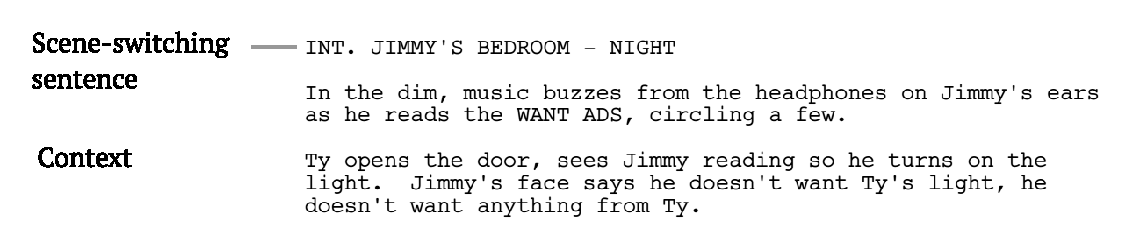
\includegraphics[scale=0.6]{figure/dataprep/script}
\caption{A Example of Script}
\label{fig:script}
\end{figure}

Figure \ref{fig:script} gives an example of what a script snippet may looks like. Usually on the top of it, there is a single sentence that specifies the location, time information for the paragraphs below it, which we would like to call as "scene-switching sentence". 
For example, in the example script, "INT. JIMMY's BEDROOM - NIGHT" is the scene-switching sentence. 
"INT" denotes this scene happens in a indoor environment. 
sometimes, "EXT" is used to denote ourdoor environment. 
In the middle of this sentence, some word phrase or sentence may be used to represent the context or scene. 
In this case, we may say this is a bedroom scene. 
Lastly, "NIGHT" or "DAY" is ued to refer the time when filmakers are shooting this script. 
When we are mining the relation between audible events and scenes, the scene-switching sentence needs to be further processed. 

Currently, there are some websites that host a collection of scripts. 
The website we used include: Simply Scripts\footnote{http://www.simplyscripts.com}, The Daily Script\footnote{http://www.dailyscript.com}, The Screenplay Database\footnote{http://www.screenplaydb.com/film/all/}, The Internet Movie Script Database(IMSDB)\footnote{http://www.imsdb.com/}, etc. 

Since the scripts are downloaded from various sites and are in different formats, we first transform the downloaded pdf or html into txt format. 
To avoid the issue of downloading the same file from different websites, the file name is checked to discard adundant scripts which have the same name with existing scripts. 
After cleaning, there are 5611 scripts in total. 

\section{Summary}
